%
% Main document
% ===========================================================================
% This is part of the document "Project documentation template".
% Authors: brd3, kaa1
%

%---------------------------------------------------------------------------
\documentclass[
a4paper,					% paper format
10pt,							% fontsize
twoside,					% double-sided
openright,				% begin new chapter on right side
notitlepage,			% use no standard title page
parskip=half,			% set paragraph skip to half of a line
]{scrreprt}					% KOMA-script report
%---------------------------------------------------------------------------

\raggedbottom
\KOMAoptions{cleardoublepage=plain}			% Add header and footer on blank pages


% Load Standard Packages:
%---------------------------------------------------------------------------
\usepackage[standard-baselineskips]{cmbright}
\usepackage[useregional]{datetime2}
\usepackage[UKenglish]{babel}
\DTMlangsetup[en-GB]{ord=raise,monthyearsep={,\space}}
\usepackage{textcomp}													% additional symbols
\usepackage{ae}																% better resolution of Type1-Fonts 
\usepackage{fancyhdr}													% simple manipulation of header and footer 
\usepackage{etoolbox}													% color manipulation of header and footer
\usepackage{graphicx}                      		% integration of images
\usepackage{float}														% floating objects
\usepackage{caption}													% for captions of figures and tables
\usepackage{booktabs}													% package for nicer tables
\usepackage{tocvsec2}													% provides means of controlling the sectional numbering
\usepackage{listings}
\usepackage{inconsolata}
\usepackage{pdflscape}
%\usepackage{tikz}
%\usepackage{pgf}
%\usepackage{pgfplots}
%\pgfplotsset{width=7cm,compat=1.16}
\usepackage{color}
\definecolor{lightgray}{rgb}{.9,.9,.9}
\definecolor{darkgray}{rgb}{.4,.4,.4}
\definecolor{purple}{rgb}{0.65, 0.12, 0.82}
\definecolor{bluekeywords}{rgb}{0.13,0.13,1}
\definecolor{greencomments}{rgb}{0,0.5,0}
\definecolor{redstrings}{rgb}{0.9,0,0}

\lstdefinelanguage{JavaScript}{
morekeywords={class, export, boolean, throw, implements, import, this, do, if, in, for, let, new, try, var, case, else, enum, eval, null, this, true, void, with, await, break, catch, class, const, false, super, throw, while, yield, delete, export, import, public, return, static, switch, typeof, default, extends, finally, package, private, continue, debugger, function, arguments, interface, protected, implements, instanceof},
sensitive=false,
comment=[l]{//},
morecomment=[s]{/*}{*/},
morestring=[b]{'},
morestring=[b]{"},
sensitive=true,
showspaces=false,
showtabs=false,
breaklines=true,
showstringspaces=false,
breakatwhitespace=true,
escapeinside={(*@}{@*)},
commentstyle=\color{greencomments},
keywordstyle=\color{bluekeywords},
stringstyle=\color{redstrings},
basicstyle=\ttfamily
}

\lstdefinelanguage{Go}{
morekeywords=[1]{break,case,chan,const,continue,default,defer,%
else,fallthrough,for,func,go,goto,if,import,interface,map,%
package,range,return,select,struct,switch,type,var},%keywords
morekeywords=[2]{append,cap,close,complex,copy,delete,imag,len,%
make,new,panic,print,println,real,recover},%functions
morekeywords=[3]{nil,true,false,iota}%constants
morekeywords=[4]{bool,byte,complex64,complex128,error,float32,%
float64,int,int8,int16,int32,int64,rune,string,uint,uint8,%
uint16,uint32,uint64,uintptr},%types
% Strings : "toto", 'toto', `toto`
morestring=[b]{"},
morestring=[b]{'},
morestring=[b]{`},
% Comments : /* comment */ and // comment
comment=[l]{//},
morecomment=[s]{/*}{*/},
% Options
sensitive=true,
showspaces=false,
showtabs=false,
breaklines=true,
showstringspaces=false,
breakatwhitespace=true,
escapeinside={(*@}{@*)},
commentstyle=\color{greencomments},
keywordstyle=\color{bluekeywords},
stringstyle=\color{redstrings},
basicstyle=\ttfamily
}

%---------------------------------------------------------------------------

% Load Math Packages
%---------------------------------------------------------------------------
\usepackage{amsmath}                    	   	% various features to facilitate writing math formulas
\usepackage{amsthm}                       	 	% enhanced version of latex's newtheorem
\usepackage{amsfonts}                      		% set of miscellaneous TeX fonts that augment the standard CM
\usepackage{amssymb}													% mathematical special characters
\usepackage{exscale}													% mathematical size corresponds to textsize
%---------------------------------------------------------------------------

% Package to facilitate placement of boxes at absolute positions
%---------------------------------------------------------------------------
\usepackage[absolute]{textpos}
\setlength{\TPHorizModule}{1mm}
\setlength{\TPVertModule}{1mm}
%---------------------------------------------------------------------------					

% Definition of Colors
%---------------------------------------------------------------------------
\definecolor{linkblue}{rgb}{0,0,0.8}            % Standard
\definecolor{darkblue}{rgb}{0,0.08,0.45}        % Dark blue
\definecolor{bfhgrey}{rgb}{0.41,0.49,0.57}      % BFH grey
%\definecolor{linkcolor}{rgb}{0,0,0.8}     			% Blue for the web- and cd-version!
\definecolor{linkcolor}{rgb}{0,0,0}        			% Black for the print-version!
%---------------------------------------------------------------------------

%---------------------------------------------------------------------------

% Set up page dimension
%---------------------------------------------------------------------------
\usepackage{geometry}
\geometry{
a4paper,
left=28mm,
right=15mm,
top=30mm,
headheight=20mm,
headsep=10mm,
textheight=242mm,
footskip=15mm
}
%---------------------------------------------------------------------------

% Makeindex Package
%---------------------------------------------------------------------------
\usepackage{makeidx}                         		% To produce index
\makeindex                                    	% Index-Initialisation
%---------------------------------------------------------------------------

% Glossary Package
%---------------------------------------------------------------------------
% the glossaries package uses makeindex
% if you use TeXnicCenter do the following steps:
%  - Goto "Ausgabeprofile definieren" (ctrl + F7)
%  - Select the profile "LaTeX => PDF"
%  - Add in register "Nachbearbeitung" a new "Postprozessoren" point named Glossar
%  - Select makeindex.exe in the field "Anwendung" ( ..\MiKTeX x.x\miktex\bin\makeindex.exe )
%  - Add this [ -s "%tm.ist" -t "%tm.glg" -o "%tm.gls" "%tm.glo" ] in the field "Argumente"
%
% for futher informations go to http://ewus.de/tipp-1029.html
%---------------------------------------------------------------------------
\usepackage[nonumberlist,acronym]{glossaries}

\newglossaryentry{BibTeX}{name={BibTeX},description={Program for the creation of 	bibliographical references and directories in \TeX or \LaTeX documents}}
\newglossaryentry{Index}{name={Index},description={Index with keywords from text}}




\newacronym{AAL2}{AAL2}{Authenticator Assurance Level 2}
\newacronym{AAL3}{AAL3}{Authenticator Assurance Level 3}
\newacronym{AAL}{AAL}{Authenticator Assurance Level}
\newacronym{AATL}{AATL}{Adobe Approved Trust List}
\newacronym{AES}{AES}{Advanced Electronic Signatures}
\newacronym{API}{API}{Application Programming Interface}
\newacronym{AVX2}{AVX2}{Advanced Vector Extensions 2}
\newacronym{BLS}{BLS}{Boneh-Lynn-Shacham}
\newacronym{CA}{CA}{Certificate Authority}
\newacronym{CAdES}{CAdES}{Cryptographic Message Syntax Advanced Electronic Signature}
\newacronym{CLR}{CLR}{.NET Common Language Runtime}
\newacronym{CMS}{CMS}{Cryptographic Message Syntax}
\newacronym{CORS}{CORS}{Cross-Origin Resource Sharing}
\newacronym{CRL}{CRL}{Certificate Revocation List}
\newacronym{CSC}{CSC}{Cloud Signature Consortium}
\newacronym{CSR}{CSR}{Certificate Signing Request}
\newacronym{CSRF}{CSRF}{Cross Site Request Forgery}
\newacronym{CSRNG}{CSRNG}{Cryptographically Secure Random Number Generator}
\newacronym{CSS}{CSS}{Cascading Stylesheets}
\newacronym{CT}{CT}{Certificate Transparency}
\newacronym{DER}{DER}{Distinguished Encoding Rules}
\newacronym{DNS}{DNS}{Domain Name System}
\newacronym{DoS}{DoS}{Denial of Service}
\newacronym{DSA}{DSA}{Digital Signature Algorithm}
\newacronym{DSS}{DSS}{Digital Signature Service}
\newacronym{ECC}{ECC}{Elliptic Curve Cryptography}
\newacronym{ECDSA}{ECDSA}{Elliptic Curve Digital Signature Algorithm}
\newacronym{Ed25519}{Ed25519}{EdDSA with Curve25519 and SHA-512}
\newacronym{EdDSA}{EdDSA}{Edwards-curved Digital Signature Algorithm}
\newacronym{eIDAS}{eIDAS}{electronic IDentification, Authentication and trust Services}
\newacronym{ETSI}{ETSI}{European Telecommunications Standards Institute}
\newacronym{EU}{EU}{European Union}
\newacronym{EUTL}{EUTL}{European Union Trust List}
\newacronym{FIDO}{FIDO}{Fast IDentity Online}
\newacronym{GMT}{GMT}{Greenwich Median Time}
\newacronym{GNU}{GNU}{GNU's Not Unix}
\newacronym{GUI}{GUI}{Graphical User Interface}
\newacronym{HKDF}{HKDF}{HMAC-based Key Derivation Function}
\newacronym{HMAC}{HMAC}{Keyed-Hash Message Authentication Code}
\newacronym{HSM}{HSM}{Hardware Security Module}
\newacronym{HTML}{HTML}{Hypertext Markup Language}
\newacronym{HTTP}{HTTP}{Hypertext Transfer Protocol}
\newacronym{HTTPS}{HTTPS}{HTTP over TLS}
\newacronym{IAL3}{IAL3}{Identity Assurance Level 3}
\newacronym{IAL}{IAL}{Identity Assurance Level}
\newacronym{ICT}{ICT}{Information and Communications Technologies}
\newacronym{IDE}{IDE}{Integrated Development Environment}
\newacronym{IDM}{IDM}{Identity and Access Management}
\newacronym{IDP}{IDP}{Identity Provider}
\newacronym{IEC}{IEC}{International Electrotechnical Commission}
\newacronym{IETF}{IETF}{Internet Engineering Task Force}
\newacronym{ISO}{ISO}{International Standards Organisation}
\newacronym{JKS}{JKS}{Java Keystore}
\newacronym{JSON}{JSON}{JavaScript Object Notation}
\newacronym{JVM}{JVM}{Java Virtual Machine}
\newacronym{JWK}{JWK}{JSON Web Key}
\newacronym{JWKS}{JWKS}{JSON Web Key Store}
\newacronym{JWS}{JWS}{JSON Web Signature}
\newacronym{JWT}{JWT}{JSON Web Token}
\newacronym{LoA}{LoA}{Level of assurance}
\newacronym{LTV}{LTV}{Long-Term Validation}
\newacronym{MAC}{MAC}{Message Authentication Code}
\newacronym{MFA}{MFA}{Multi-factor authentication}
\newacronym{NIST}{NIST}{National Institute of Standards and Technology}
\newacronym{OASIS}{OASIS}{Organisation for the Advancement of Structured Information Standards}
\newacronym{OCSP}{OCSP}{Online Certificate Status Protocol}
\newacronym{OIDC}{OIDC}{OpenID Connect}
\newacronym{OpenAPI}{OpenAPI}{Open Application Programming Interface}
\newacronym{PAdES}{PAdES}{Portable Document Format Advanced Electronic Signature}
\newacronym{PDF}{PDF}{Portable Document Format}
\newacronym{PEM}{PEM}{Privacy-Enhanced Mail}
\newacronym{PIN}{PIN}{Personal Identification Number}
\newacronym{PKCS7}{PKCS7}{Public Key Cryptography Standard 7}
\newacronym{PKCS10}{PKCS10}{Public Key Cryptography Standard 10}
\newacronym{PKCS}{PKCS}{Public Key Cryptography Standard}
\newacronym{PKI}{PKI}{Public Key Infrastructure}
\newacronym{PKS12}{PKS12}{Public-Key Cryptograpy Standards}
\newacronym{POC}{POC}{Proof Of Concept}
\newacronym{POJOs}{POJOs}{Plain old Java object}
\newacronym{PSS}{PSS}{Probabilistic Signature Scheme}
\newacronym{QES}{QES}{Qualified Electronic Signatures}
\newacronym{RA}{RA}{Registration Authority}
\newacronym{REST}{REST}{Representational State Transfer}
\newacronym{RFC}{RFC}{Request For Comments}
\newacronym{RNG}{RNG}{Random Number Generator}
\newacronym{RSA-PSS}{RSA-PSS}{RSA Probabilistic Signature Scheme}
\newacronym{RSA}{RSA}{Rivest-Shamir-Adleman}
\newacronym{SAD}{SAD}{Signature activation data}
\newacronym{SDK}{SDK}{Software Development Kit}
\newacronym{SHA-256}{SHA-256}{Secure Hash Algorithm 2 with 256-bit output length}
\newacronym{SHA-2}{SHA-2}{Secure Hash Algorithm 2}
\newacronym{SHA}{SHA}{Secure Hash Algorithm}
\newacronym{SIM}{SIM}{Subscriber Identity Module}
\newacronym{SMS}{SMS}{Short Message System}
\newacronym{SOAP}{SOAP}{Simple Object Access Protocol}
\newacronym{SPA}{SPA}{Single Page Application}
\newacronym{TLS}{TLS}{Transport Layer Security}
\newacronym{TOTP}{TOTP}{Time-based One Time Password}
\newacronym{TSA}{TSA}{Time Stamping Authority}
\newacronym{TSS}{TSS}{Timestamping Service}
\newacronym{UI}{UI}{User Interface}
\newacronym{UML}{UML}{Unified Modeling Language}
\newacronym{URI}{URI}{Unique Resource Identifier}
\newacronym{USB}{USB}{Universal Serial Bus}
\newacronym{VM}{VM}{Virtual Machine}
\newacronym{WASM}{WASM}{WebAssembly}
\newacronym{XAdES}{XAdES}{XML Advanced Electronic Signatures}
\newacronym{XML}{XML}{Extensible Markup Language}
\newacronym{BFH}{BFH}{Bern University of Applied Sciences}
\newacronym{SLF4J}{SLF4J}{Simple Logging Facade for Java}
\newacronym{CIO}{CIO}{Coroutine-based I/O}
\newacronym{TSP}{TSP}{Time-stamp Protocol}
\newacronym{DOM}{DOM}{Document Object Model}
\newacronym{FSF}{FSF}{Free Software Foundation}
\newacronym{JAR}{JAR}{Java Archive}
\newacronym{JRE}{JRE}{Java Runtime Environment}
\newacronym{JS}{JS}{JavaScript}
\newacronym{DI}{DI}{Dependency Injection}
\newacronym{CI}{CI}{Continuous Integration}
\newacronym{JOSE}{JOSE}{JavaScript Object Signing and Encryption}
\newacronym{VCS}{VCS}{Version Control System}
\newacronym{URL}{URL}{Uniform Resource Locator}

\makeglossaries
% Hyperref Package (Create links in a pdf)
%---------------------------------------------------------------------------
\usepackage[
pdftex,ngerman,bookmarks,plainpages=false,pdfpagelabels,
backref = {false},										% No index backreference
colorlinks = {true},                  % Color links in a PDF
hypertexnames = {true},               % no failures "same page(i)"
bookmarksopen = {true},               % opens the bar on the left side
bookmarksopenlevel = {0},             % depth of opened bookmarks
pdftitle = {Remote Signing Service},	   	% PDF-property
pdfauthor = {brd3},        					  % PDF-property
pdfsubject = {LaTeX Template},        % PDF-property
linkcolor = {linkcolor},              % Color of Links
citecolor = {linkcolor},              % Color of Cite-Links
urlcolor = {linkcolor},               % Color of URLs
]{hyperref}
%---------------------------------------------------------------------------

% Intro:
%---------------------------------------------------------------------------
\begin{document}                              	% Start Document
    \settocdepth{section}														% Set depth of toc
    \pagenumbering{roman}
    %---------------------------------------------------------------------------

    \providecommand{\heading}{Remote Signing Service}		%  Insert Title of Thesis here					% Titel der Arbeit aus Datei titel.tex lesen

    % Set up header and footer
    %---------------------------------------------------------------------------
    \makeatletter
    \patchcmd{\@fancyhead}{\rlap}{\color{bfhgrey}\rlap}{}{}		% new color of header
    \patchcmd{\@fancyfoot}{\rlap}{\color{bfhgrey}\rlap}{}{}		% new color of footer
    \makeatother

    \fancyhf{}																		% clean all fields
    \fancypagestyle{plain}{												% new definition of plain style
    \fancyfoot[OR,EL]{\footnotesize \thepage} 	% footer right part --> page number
    \fancyfoot[OL,ER]{\footnotesize \heading }	% footer even page left part
    }

    \renewcommand{\chaptermark}[1]{\markboth{\thechapter.  #1}{}}
    \renewcommand{\headrulewidth}{0pt}				% no header stripline
    \renewcommand{\footrulewidth}{0pt} 				% no bottom stripline

    \pagestyle{plain}
    %---------------------------------------------------------------------------


    % Title Page and Abstract
    %---------------------------------------------------------------------------
    %
% Project documentation template
% ===========================================================================
% This is part of the document "Project documentation template".
% Authors: brd3, kaa1
%

\begin{titlepage}


% BFH-Logo absolute placed at (28,12) on A4 and picture (16:9 or 15cm x 8.5cm)
% Actually not a realy satisfactory solution but working.
%---------------------------------------------------------------------------
\setlength{\unitlength}{1mm}
\begin{textblock}{20}[0,0](28,12)
	
\includegraphics[scale=1.0]{images/BFH_Logo_B.png}
\end{textblock}

% Institution / titel / subtitel / authors / experts:
%---------------------------------------------------------------------------
\begin{flushleft}

\vspace*{21mm}

\fontsize{26pt}{40pt}\selectfont 
\heading				\\							% Read heading from file leader/title.tex
\vspace{2mm}

\fontsize{16pt}{24pt}\selectfont\vspace{0.3em}
Accessible Electronic Signatures for Everybody 			\\				% Insert subheading
\vspace{5mm}

\fontsize{10pt}{12pt}\selectfont
\textbf{Bachelor Thesis by Gabor Tanz and Patrick Hirt} \\		% Insert text
\vspace{7mm}

% Abstract (eingeben):
%---------------------------------------------------------------------------
\begin{textblock}{150}(28,100)
\fontsize{10pt}{12pt}\selectfont
    TODO abstract TODO
\end{textblock}

\begin{textblock}{150}(28,225)
\fontsize{10pt}{17pt}\selectfont
\begin{tabbing}
xxxxxxxxxxxxxxx\=xxxxxxxxxxxxxxxxxxxxxxxxxxxxxxxxxxxxxxxxxxxxxxx \kill
Degree course:	\> [z.B. Electrical and Communication Engineering]	\\		% insert name of degree course
Authors:		\> [Test Peter, M\"uster R\"os\"a]		\\					% insert names
Tutor:	\> [Dr.~Xxxx Xxxx, Dr.~Yyyy Yyyy]		\\							% insert names
Constituent:	\> [Wwwww AG]					\\							% insert names
Experts:		\> [Dr.~Zzzz Zzzz]				\\							% insert names
Date:			\> \versiondate					\\							% read from file leader/version.tex
\end{tabbing}

\end{textblock}
\end{flushleft}

\begin{textblock}{150}(28,280)
\noindent 
\color{bfhgrey}\fontsize{9pt}{10pt}\selectfont
Berner Fachhochschule | Haute \'ecole sp\'ecialis\'ee bernoise | Bern University of Applied Sciences
\color{black}\selectfont
\end{textblock}


\end{titlepage}

%
% ===========================================================================
% EOF
%
		% activate for frontpage without picture
    %%
% Project documentation template
% ===========================================================================
% This is part of the document "Project documentation template".
% Authors: brd3, kaa1
%

\begin{titlepage}


% BFH-Logo absolute placed at (28,12) on A4 and picture (16:9 or 15cm x 8.5cm)
% Actually not a realy satisfactory solution but working.
%---------------------------------------------------------------------------
\setlength{\unitlength}{1mm}
\begin{textblock}{20}[0,0](28,12)
	
\includegraphics[scale=1.0]{images/BFH_Logo_B.png}
\end{textblock}

\begin{textblock}{154}(28,48)
	\begin{picture}(150,2)
		\put(0,0){\color{bfhgrey}\rule{150mm}{2mm}}
	\end{picture}
\end{textblock}

\begin{textblock}{154}[0,0](28,50)
	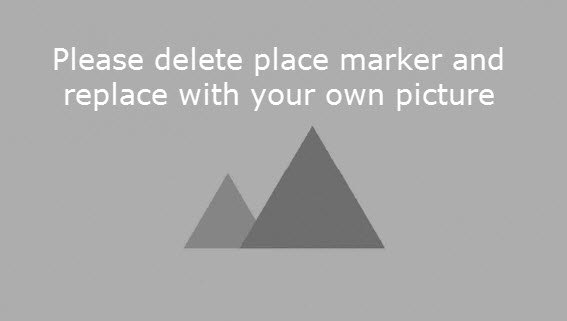
\includegraphics[scale=1.0]{images/placemarker.jpg}			% define cover picture
\end{textblock}

\begin{textblock}{154}(28,135)
	\begin{picture}(150,2)
		\put(0,0){\color{bfhgrey}\rule{150mm}{2mm}}
	\end{picture}
\end{textblock}
\color{black}

% Institution / titel / subtitel / authors / experts:
%---------------------------------------------------------------------------
\begin{flushleft}

\vspace*{115mm}

\fontsize{26pt}{28pt}\selectfont 
\heading				\\							% Read heading from file leader/title.tex
\vspace{2mm}

\fontsize{16pt}{20pt}\selectfont\vspace{0.3em}
Place your subheading here 			\\				% Insert subheading
\vspace{5mm}

\fontsize{10pt}{12pt}\selectfont
\textbf{Description of thesis (semester- / Bachelor thesis / etc.)} \\		% Insert text
\vspace{3mm}

% Abstract (eingeben):
%---------------------------------------------------------------------------
\begin{textblock}{150}(28,190)
\fontsize{10pt}{12pt}\selectfont
[Insert short text (abstract) if desired] \\ 
This document serves as a template for the compilation of reports according to the guidelines of the BFH. The template is written in LATEX and supports the automatic writing of various directories, references, indexing and glossaries. This small text is a summary of this document with a length of 4 to max. 8 lines. \\ 
The cover picture may be turned on or off in the lines 157/158 of the file template.tex.
\end{textblock}

\begin{textblock}{150}(28,225)
\fontsize{10pt}{17pt}\selectfont
\begin{tabbing}
xxxxxxxxxxxxxxx\=xxxxxxxxxxxxxxxxxxxxxxxxxxxxxxxxxxxxxxxxxxxxxxx \kill
Degree course:	\> [z.B. Electrical and Communication Engineering]	\\		% insert name of degree course
Authors:		\> [Test Peter, M\"uster R\"os\"a]		\\					% insert names
Tutor:	\> [Dr.~Xxxx Xxxx, Dr.~Yyyy Yyyy]		\\							% insert names
Constituent:	\> [Wwwww AG]					\\							% insert names
Experts:		\> [Dr.~Zzzz Zzzz]				\\							% insert names
Date:			\> \versiondate					\\							% read from file leader/version.tex
\end{tabbing}

\end{textblock}
\end{flushleft}

\begin{textblock}{150}(28,280)
\noindent 
\color{bfhgrey}\fontsize{9pt}{10pt}\selectfont
Berner Fachhochschule | Haute \'ecole sp\'ecialis\'ee bernoise | Bern University of Applied Sciences
\color{black}\selectfont
\end{textblock}


\end{titlepage}

%
% ===========================================================================
% EOF
%
		% activate for frontpage with picture
    \cleardoubleemptypage
    \setcounter{page}{1}
    \cleardoublepage
    \phantomsection
    \cleardoubleemptypage
    %---------------------------------------------------------------------------

    % Table of contents
    %---------------------------------------------------------------------------
    \tableofcontents
    \cleardoublepage
    %---------------------------------------------------------------------------

    % Main part:
    %---------------------------------------------------------------------------
    \pagenumbering{arabic}

    \chapter{Objectives}
\label{ch:objectives}

\subsection{Main Objective}\label{subsec:main-objective}
The implementation consists of the remote signing service itself in the form of a \gls{REST} \gls{API},
and a cross-platform frontend authenticating the users through a trusted \gls{OIDC} \gls{IDP}.
This frontend uses the \gls{REST} \gls{API} for signing the users' files.
On top of that, it offers offline verification of existing signatures on desktop operating systems.

\section{Previous Works}
\label{section:previousworks}

We build upon our previous work of Project 2~\cite{projekt2}, where we specified the authentication process
for qualified signatures, non-qualified batch signatures, the signature file format,
as well as - to our knowledge - pioneering the secure integration of a digital signature with an \gls{OIDC} ID token without requiring any change to the \gls{IDP}.

\section{Backend}
\label{section:backend}

The server is the centrepiece of the service, where the actual signatures are being created.
It depends on the \gls{IDP} for authenticating its users.
In our implementation, we will aim to protect the private keys by using a \gls{HSM}.

\section{Frontend}
\label{section:frontend}

The frontend must be cross-platform, where cross-platform means supporting the desktop operating systems
GNU/Linux, Microsoft Windows and Apple MacOS as well as the mobile phone operating systems Google Android and Apple iOS.
The frontend must support authentication through the \gls{IDP}, creating signatures through the backend, as well as verifying them.
Verification must be available online as well as offline, except for the mobile version, where offline verification is not required.

\section{Comparison With Existing Solutions}
\label{section:comparison}

The Cloud Signature Consortium standardised a remote signing service with OIDC/oAuth.
Adobe has made an implementation of this standard.
The goal is to learn how this implementation works and compare it with our solution, with a focus on security.

\section{Evaluation of the Yubikey HSM for Signing Service}
\label{section:evaluateyubikey}

In order to provide a secure solution for the signing keys, we will evaluate the Yubikey HSM 2.
This would allow us to avoid having the signing keys on the filesystem, thus strongly improving the security of our solution.



    \chapter{Actors}
\label{ch:actors}

Actors specify a role played by a user or a system for the purposes of a clearer definition.
In this chapter, we will outline the actors in our system.

\begin{landscape}
	\topskip0pt
	\vspace*{\fill}
	\section{Big Picture}
	\begin{figure}[H]
		\begin{center}
			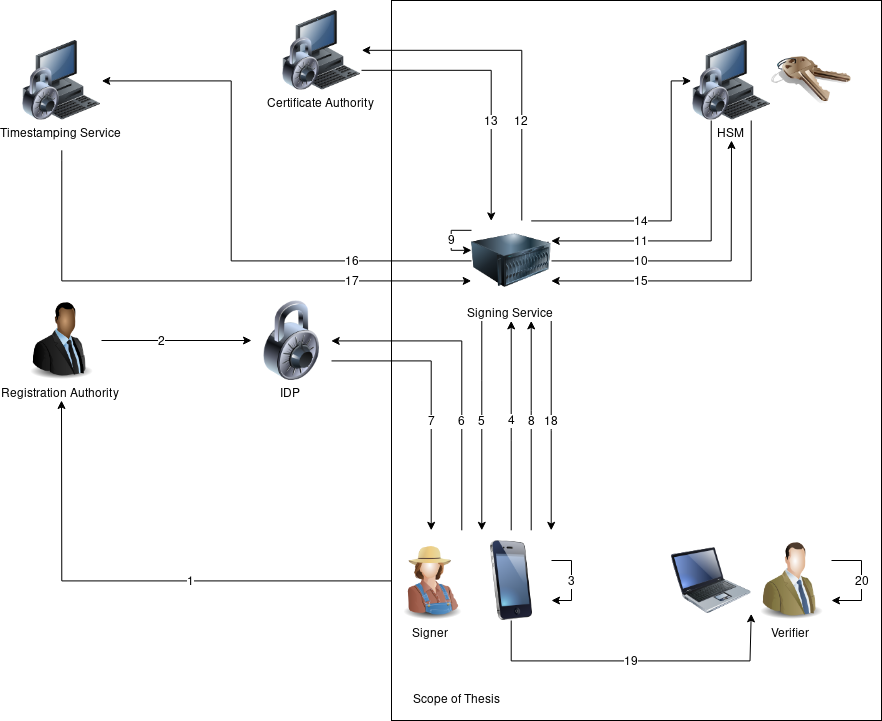
\includegraphics[scale=0.6]{images/BigPicture.png}
			\caption{Big Picture}
			\label{fig:bigpicture}
		\end{center}
	\end{figure}
	\vspace*{\fill}
\end{landscape}

\subsubsection{Steps}
\begin{enumerate}
	\item Registration of identity with RA (Authenticator)
	\item Propagate identity to IDP (Identifier)
	\item Generate document hash
	\item Send hash to signing service
	\item Receive OIDC redirect to IDP
	\item Login to IDP
	\item Receive ID token
	\item Send ID token to signing service
	\item Verify ID token
	\item Request signing key CSR from HSM
	\item Receive CSR
	\item Send CSR to CA
	\item Receive signed Certificate
	\item Request signature from HSM
	\item Receive signature
	\item Request timestamp from TSS
	\item Receive timestamp
	\item Send signature to signer
	\item Send document and signature to Verifier/Receiver
	\item Verify document and signature
\end{enumerate}


\section{The Signer}
\label{sec:actorsigner}
The Signer is the person who wishes to have the signing server sign a document in their name.
For example, a medical professional issuing a prescription for medication to a patient.

\section{The Verifier}
\label{sec:actorverifier}
The Verifier is the person who wishes to verify the integrity and authorship of a document.
For example, the pharmacist whom the patient gives the prescription to (as previously authored and signed by The Signer as specified in section~\ref{sec:actorsigner}) in order to purchase the medication prescribed by the medical professional.

\section{The Authenticator}
\label{sec:actorauthenticator}
The Authenticator is the system who authenticates The Signer as specified in section~\ref{sec:actorsigner}.
In \gls{NIST} terminology~\cite{nistdigitalidentityguidelines}, this is the entity establishing the \gls{IAL}.
In order for The Authenticator to be able to authenticate The Signer,
they must have been registered with The Authenticator by The Identifier as specified in section~\ref{sec:authoridentifier}.

\section{The Identifier}
\label{sec:authoridentifier}
The Identifier is the system or person who asserts the identity of The Signer.
In order for the signing service to issue qualified signatures as defined by relevant Swiss legislation~\cite{zertes} and Swiss Federal Council regulations~\cite{vzertes},
the identity must be proven in-person using a government-issued photographic identification document such as a passport.

\section{The Signing Service}
\label{sec:signingservice}
The Signing Service is the system who actually creates the signatures on behalf of the user.
It generates the signing keys and requests the \gls{CA}~\ref{sec:ca} to sign them.

\section{The Certificate Authority}
\label{sec:ca}
The \gls{CA} is the system who signs the signing keys generated by the Signing Service~\ref{sec:signingservice}.

    \chapter{Functional Requirements}
\label{ch:functionalrequirements}

\section{Terminology}

As always, the usual modal verbs are to be interpreted as in RFC 2119~\cite{rfc2119}.

\subsection{Practically Impossible}
"Practically impossible" means the probability of it being possible is not zero, but so small for it not to matter in practice.
An example for this would be finding the prime factors of the product of two carefully chosen 1024 bit numbers within 24 hours.

\subsection{Being made difficult}
"Made difficult" means something far from impossible for someone with near-unlimited resources like a state actor,
but extremely difficult if not impossible even for a highly skilled single person with the resources expected for a single person.
For example, stealing a smart card from someone and misusing the contained private key.

\section{Signature Requirements}
\label{sec:signaturerequirements}
\subsection{Authenticity}
\label{subsec:authenticity}
It must be practically impossible for anyone to forge a signature without it being detected upon signature verification.

\subsection{Integrity}\label{subsec:integrity}
It must be practically impossible for anyone to modify a signed document without being detected upon signature verification.
A secure hash algorithm must be used for hashing the document.
Secure means the algorithm to be pre-image as well as collision-resistant as validated by the \gls{NIST} Cryptographic Algorithm Validation Program~\cite{nistcavp}.

\subsection{Verifiability}\label{subsec:verifiability}
Anyone must be able to verify the authenticity of a signature and the integrity of the signed document.

\subsection{Non-repudiation}\label{subsec:non-repudiation}
It must be practically impossible for anyone to deny having signed a document.

\subsection{Long-Term Validation}\label{subsec:long-term-validation}
Signatures must be suitable for \gls{LTV} using an RFC3161~\cite{rfc3161} timestamp.

\subsection{Secure Coupling of Authentication and Signature}\label{subsec:secure-coupling-of-authentication-and-signature}
It must be practically impossible for anyone to abuse a stolen \gls{OIDC} ID token to sign a document other than intended by The Signer.

\subsection{Authentication Protocol}\label{subsec:authentication-protocol}
Standard \gls{OIDC} must be used for authenticating The Signer as specified in the standard~\cite{oidc}.

\subsection{Supported File Formats}\label{subsec:supported-file-formats}
It must be possible to sign any file, regardless of its format.

\subsection{Bulk Signatures}\label{subsec:bulk-signatures}
For qualified signatures, it must be possible to sign more than one document at once.

For advanced signatures, it may be possible to sign several documents one after the other without requiring re-authentication.

\subsection{Device-local Hashing of Documents}\label{subsec:local-hashing-of-documents}
In order to ensure privacy and protection of information as required by~\ref{subsec:protection-of-information},
documents to be signed must not leave the users' device.
For webinterfaces, this means that the document must be hashed in the browser itself.

\section{Signature Server Requiremenents}
\label{sec:signatureserverrequirements}
\subsection{CA Key Security}\label{subsec:ca-key-security}
Technical measures must be taken to make it difficult for the private keys of the signing \gls{CA} to be stolen.

\subsection{Signing Key Security}\label{subsec:signing-key-security}
Technical measures must be taken to make it difficult to steal the private keys generated on behalf of the users.

\subsection{No unauthorised identity delegation}\label{subsec:no-unauthorised-identity-delegation}
It must be practically impossible for the signing server to create a signature on its own.

\subsection{Random Number Generation}\label{subsec:random-number-generation}
The \gls{RNG} used for generating signatures must be a cryptographically secure.

\subsection{REST API}\label{subsec:rest-api}
The Signature Server must offer a \gls{REST} \gls{API} that can be used by third parties to interface with the signing service,
for example in order to implement custom frontends or to include it as part of their product,
or for users that don't like \gls{GUI}s.

\chapter{Non-Functional Requirements}
\label{ch:nonfunctionalrequirements}

\subsection{Efficient Signature File Format}\label{subsec:efficient-signature-file-format}
The file format for the signature file shall be based on our previous work~\cite{projekt2}.

\subsection{Protection of Information}\label{subsec:protection-of-information}
Information not strictly required by the party in order to fulfil their function must not be disclosed to the aforementioned party.
In particular, the document to be signed must not be disclosed to the signing server nor to the \gls{IDP}.
The \gls{IDP} must not learn of the document hash.
More generally, every actor must not have any more information disclosed to it than is necessary for them to perform their function.

\subsection{Offline Validation}\label{subsec:offline-validation}
The Verifier must be enabled to verify signatures without an active internet connection using a desktop or laptop computer running GNU/Linux, MacOS or Windows.

\section{IDP Requirements}\label{sec:idp-requirements}
Anything related to the \gls{IDP} is out of scope for our thesis, except for specifying what we require of the same.
We assume to be using an existing, \gls{OIDC}-conforming \gls{IDP} providing the required registration and authentication levels.

\subsection{Support for OIDC}\label{subsec:support-for-oidc}
The \gls{IDP} must support standard \gls{OIDC} as specified in the standard~\cite{oidc}.


\subsection{Levels of Assurance}\label{subsec:levels-of-assurance}
The \gls{IDP} must support \gls{AAL} 2 authentication for advanced signatures, and \gls{AAL} 3 authentication for qualified signatures as specified in the \gls{NIST} publication~\cite{nistdigitalidentityguidelines}.

\section{Prioritisation of Requirements}
\label{sec:prioritisation}
\begin{longtable}{p{12cm}|p{2.5cm}}
    \textbf{Requirement} & \textbf{Prioritisation}\\
    \hline
    Authenticity of signature~(\ref{subsec:authenticity}) & Must\\
    Integrity of document~(\ref{subsec:integrity}) & Must\\
    Verifiability of signature~(\ref{subsec:verifiability}) & Must\\
    Non-repudiation~(\ref{subsec:non-repudiation}) & Must\\
    Secure coupling of authentication and signature~(\ref{subsec:secure-coupling-of-authentication-and-signature}) & Must\\
    Authentication protocol~(\ref{subsec:authentication-protocol}) & Must\\
    Supported file formats~(\ref{subsec:supported-file-formats}) & Must\\
    Signing key security~(\ref{subsec:signing-key-security}) & Must\\
    No unauthorised identity delegation~(\ref{subsec:no-unauthorised-identity-delegation}) & Must\\
    Random number generation~(\ref{subsec:random-number-generation}) & Must\\
    \gls{REST} \gls{API}~(\ref{subsec:rest-api}) & Must\\
    Offline validation~(\ref{subsec:offline-validation}) & Must\\
    Protection of information~(\ref{subsec:protection-of-information}) & Optional\\
    Device-local hashing of documents~(\ref{subsec:local-hashing-of-documents}) & Optional\\
    Efficient signature file format~(\ref{subsec:efficient-signature-file-format}) & Optional\\
    \gls{CA} key security~(\ref{subsec:ca-key-security}) & Optional\\
    Bulk signatures~(\ref{subsec:secure-coupling-of-authentication-and-signature}) & Optional\\
    Long-term validation~(\ref{subsec:long-term-validation}) & Optional\\
    \caption{Prioritisation of Requirements}
\end{longtable}

    \chapter{Use-Cases}\label{ch:usecases}

\section{Document Signing}\label{sec:document-signing}

\subsection{Prerequisites}\label{subsec:prerequisites}
The following prerequisites have to be fulfilled in order for the following use cases to work:
\begin{enumerate}
    \item The user (actor~\ref{sec:actorsigner}) has registered with the \gls{RA} (actor~\ref{sec:authoridentifier}) and is known to the \gls{IDP}~(actor~\ref{sec:actorauthenticator})
    \item The user has created and readied a document file to be signed
\end{enumerate}

\subsection{Interactive Qualified Signatures}\label{subsec:interactive-qualified-signatures}
\subsubsection{Steps}
The user performs the following steps:
\begin{enumerate}
    \item Opens the webinterface of the signing service (actor~\ref{sec:actorsigningservice}) on their device
    \item Selects the document file to be hashed
    \item Selects the preferred \gls{IDP} out of a list of trusted \gls{IDP}s, if multiple \gls{IDP}s are configured
    \item Gets redirected to the \gls{IDP}s login page
    \item Authenticates with the \gls{IDP}
    \item Gets redirected back to the signing service
    \item Receives the signature as a file download
    \item Saves the signature file to their device
\end{enumerate}

\subsubsection{Result}
The user has received a signature file for the document file they wanted to sign.

\subsection{Bulk Advanced Signatures}\label{subsec:bulk-advanced-signatures}
In some cases, users might wish to sign document files all day long without being required to authenticate with the \gls{IDP} for every document.
In this case the authentication will be cached for a certain duration without needing to re-authenticate for each document.
In this mode only advanced signatures can be created.

From the users' point of view, it works like this:
\begin{enumerate}
    \item The user opens the webinterface of the signing service on their device
    \item If implemented, they click the button for authentication for batch advanced signatures
    \item Gets redirected to the \gls{IDP}
    \item Authenticates with the \gls{IDP}
    \item Gets redirected back to the signing service
    \item For the duration of the authentication, the user can now submit document files to be signed,
        receiving the corresponding signature files, without the need to reauthenticate.
\end{enumerate}
\subsubsection{Result}
The user receives advanced signature files for each of the document files they submit for signing for the duration of the authentication.


\section{Signature Validation}\label{sec:signature-validation}

\subsection{Prerequisites}\label{subsec:prerequisites2}
The following prerequisites have to be fulfilled in order for the following use cases to work:
\begin{enumerate}
    \item A signature file has been created beforehand as described in~\ref{subsec:interactive-qualified-signatures}.
\end{enumerate}

\subsection{Offline Validation}\label{subsec:offline-validation2}
The signatures can be verified offline with just the document file, the signature file and the verification program.
This mode will only be supported on desktop operating systems (GNU/Linux, Windows, macOS), not on mobile devices (Android, iOS).

\subsubsection{Steps}
The user performs the following steps:
\begin{enumerate}
    \item The user opens the verification program
    \item The user selects the document file and corresponding signature file and submits it to the verification program
    \item The program verifies the signature and displays the result
\end{enumerate}
\subsubsection{Result}
The user knows whether the signature is genuine and whether the document integrity is guaranteed.

\subsection{Online Validation}\label{subsec:semi-online-validation}
For mobile clients a website will be provided to validate the signature by providing the document and the signature.

\subsubsection{Prerequisites}
In addition to the prerequisites specified in subsection~\ref{subsec:prerequisites2},
it is necessary for the user to have opened the signature services' verification web page in their browser beforehand
so that it is available to the user without connecting to the server again.
This is why we call it semi-online.
For example, the user opens the web browser on their mobile phone and loads the verification page.
Then they board an aeroplane and turn on aeroplane mode.
After takeoff, they decide to validate a signature.
Then they proceed as follows:

\subsubsection{Steps}
The user performs the following steps:
\begin{enumerate}
    \item The user opens the web browser where the verification page is still available
    \item The user selects the document file and corresponding signature file and submits it to the verification website
    \item The website verifies the signature in-browser (without needing to connect to any additional servers) and displays the result
\end{enumerate}
\subsubsection{Result}
The user knows whether the signature is genuine and whether the document integrity is guaranteed.

    \chapter{Project Management}
\label{ch:projectmanagement}

\section{Project Method}
\label{sec:projectmethod}
We will be using the SCRUM process for organising our work.
This means splitting the work packages into stories and scheduling for completion in sprints.
Sprints shall last two weeks. At the end of every sprint the progress is reviewed with the advisors and the next sprint is planned.

\section{Project Timeline}
\label{sec:projecttimeline}
Since we know in advance the timeframes within we must complete our work, we created the following project timeline.

\begin{landscape}
\topskip0pt
\vspace*{\fill}
	\begin{figure}[H]
	\begin{center}
		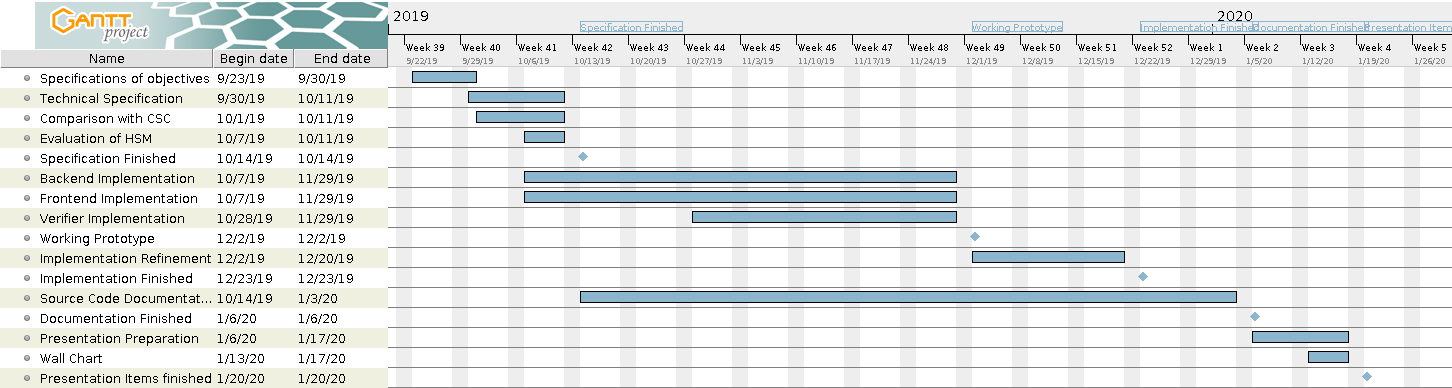
\includegraphics[scale=0.5]{images/Projectplan.png}
		\caption{Project timeline}
		\label{fig:projecttimeline}
	\end{center}
	\end{figure}
\vspace*{\fill}
\end{landscape}

\section{Work Packages}
\label{sec:workpackages}

\subsection{Specification of Objectives}\label{subsec:specification-of-objectives}
The objectives of our thesis will be specified.
This included functional and non-functional requirements.

\subsection{Technical Specification}\label{subsec:technical-specification}
The requirements defined in the objectives will be mapped to concrete technology choices.
Also the choice of languages and frameworks will be explained.

\subsection{Comparison with CSC Implementation}\label{subsec:comparison-with-csc-implementation}
We will compare our Specification with the Remote Signing Standard specified by the \gls{CSC}.

\subsection{Evaluation of Yubikey HSM}\label{subsec:evaluation-of-yubikey-hsm}
We will evaluate how we can use the Yubikey HSM for our Signature Service.

\subsection{Backend Implementation}\label{subsec:backend-implementation}
The backend consisting of the Signing Service and the OIDC Coupling with the IDP will be implemented.

\subsection{Frontend Implementation}\label{subsec:frontend-implementation}
The frontend consisting of the Hashing and UI will be implemented.

\subsection{Standalone Verifier Implementation}\label{subsec:standalone-verifier-implementation}
The application for the offline verification of the signature will be implemented.

\subsection{Implementation Refinement}\label{subsec:implementation-refinement}
After the working prototype, eventual bugs will be fixed and optional goals will be implemented.

\subsection{Source Code Documentation}\label{subsec:source-code-documentation}
We will document the source code.

\subsection{Presentation}\label{subsec:presentation}
We will create the slides and prepare the presentation.

\subsection{Wall Chart and Article}\label{subsec:wall-chart-and-article}
We will create a wall chart and short article describing our work.

\subsection{Video}\label{subsec:video}
We will create a short video introducing our problem.
    %---------------------------------------------------------------------------

    % Glossary
    %---------------------------------------------------------------------------
    \cleardoublepage
    \phantomsection
    \addcontentsline{toc}{chapter}{Glossay}
    %\renewcommand{\glossaryname}{Glossay}
    \printglossary
    %---------------------------------------------------------------------------

    % Bibliography
    %---------------------------------------------------------------------------
    \cleardoublepage
    \phantomsection
    \addcontentsline{toc}{chapter}{Bibliography}
    \bibliographystyle{IEEEtranS}
    \bibliography{database/bibliography}{}
    \printglossaries
    %---------------------------------------------------------------------------

    % Listings
    %---------------------------------------------------------------------------
    \cleardoublepage
    \phantomsection
    \addcontentsline{toc}{chapter}{List of figures}
    \listoffigures
    \cleardoublepage
    \phantomsection
    \addcontentsline{toc}{chapter}{List of tables}
    \listoftables
    \lstlistoflistings
    %---------------------------------------------------------------------------

    % Index
    %---------------------------------------------------------------------------
    \cleardoublepage
    \phantomsection
    \addcontentsline{toc}{chapter}{Index}
    \printindex
    %---------------------------------------------------------------------------


    %---------------------------------------------------------------------------
\end{document}

